% vim: set foldmethod=marker foldlevel=0:

\documentclass[a4paper]{article}
\usepackage[UKenglish]{babel}

\usepackage{preamble}

\usepackage{graphicx}
\graphicspath{ {./imgs/} }

\fancyhead[L]{MA139 Assignment 3}
\title{MA139 Analysis 2, Assignment 3}
\colorlet{questionbodycolor}{cyan!50}

\begin{document}

\maketitle

\setlength{\parindent}{0em}
\setlength{\parskip}{1em}

% {{{ Q1
\question{1}

\begin{questionbody}
Let $f \colon (-1, 1) \to \R$ be the function defined by \[
f(t) = \log\l( \f{1+t}{1-t} \r) - 2t = \log(1+t) - \log(1-t) - 2t.
\] Assuming knowledge of the derivative of $\log$ show that $f$ is increasing on $(-1, 1)$.

Deduce that $\ds\log\l( \f{1+t}{1-t} \r) \ge 2t$ for $0 \le t < 1$.

Prove that if $x > 0$ then $\ds\log\l( 1 + \f1x \r) \ge \f2{2x+1}$.

Deduce that for each positive $x$, $\ds\l( 1 + \f1x \r)^{x + \f12} \ge \e$.

You already saw that $\ds\l( 1 + \f1x \r)^{x + 1} \ge \e$.

Draw a graph of the two functions $\ds x \mapsto \l( 1 + \f1x \r)^{x + \f12}$ and $\ds x \mapsto \l( 1 + \f1x \r)^{x + 1}$ for $x > 0$ and the horizontal line $y = \e$ to see how much more accurate the new inequality is. (This gives you some idea of the power of the derivative.)
\end{questionbody}

\begin{align*}
f'(t) &= \f1{1+t} - (-1)\f1{1-t} - 2\\[1ex]
&= \f{1-t + 1+t}{1-t^2} - 2\\[1ex]
&= \f{2 - 2(1-t^2)}{1-t^2}\\[1ex]
&= \f{2t^2}{1-t^2}
\end{align*}

In the range $t \in (-1, 1)$, $t^2 \in (0, 1)$. Therefore $2t^2 > 0$ and $1 - t^2 > 0$, so $f'(t) > 0$. Therefore $f(t)$ is increasing for $t \in (-1, 1)$.

$f(0) = \log(1) - 0 = 0$ and since $f(t)$ is increasing, $f(t) \ge 0$ for $t \in [0, 1)$. Therefore $\log\l( \f{1+t}{1-t} \r) - 2t \ge 0 \implies \log\l( \f{1+t}{1-t} \r) \ge 2t$ for $0 \le t < 1$ as required.

Let $t = \df1{2x+1}$. Then \begin{align*}
\f{1+t}{1-t} &= \f{1 + \f1{2x+1}}{1 - \f1{2x+1}}\\[1ex]
&= \f{2x + 1 + 1}{2x + 1 - 1}\\[1ex]
&= \f{2x + 2}{2x}\\[1ex]
&= 1 + \f1x
\end{align*}
Therefore $$\log\l( \f{1+t}{1-t} \r) \ge 2t \implies \log\l( 1 + \f1x \r) \ge \f2{2x+1}$$
for the condition \begin{align*}
0 &\le t < 1\\[1ex]
0 &\le \f1{2x+1} < 1\\[1ex]
0 &\le 1 < 2x + 1\\[1ex]
% 1 &< 2x + 1\\[1ex]
0 &< 2x\\[1ex]
0 &< x\\[1ex]
\end{align*}

Then \begin{align*}
\log\l( 1 + \f1x \r) &\ge \f2{2x+1}\\[1ex]
(2x+1) \log\l( 1 + \f1x \r) &\ge 2\\[1ex]
(x + \f12) \log\l( 1 + \f1x \r) &\ge 1\\[1ex]
\log\l( \l( 1 + \f1x \r)^{x + \f12} \r) &\ge 1\\[1ex]
\l( 1 + \f1x \r)^{x + \f12} &\ge \e\\[1ex]
\end{align*}

\begin{center}
	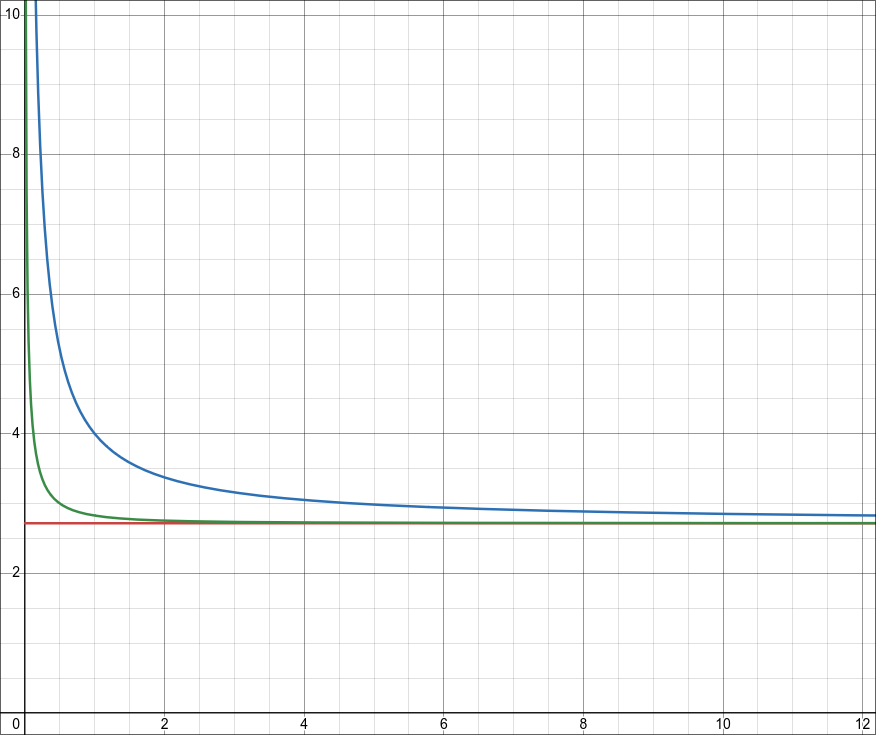
\includegraphics[scale=0.3]{Q1-graph.png}
\end{center}

% }}}

% {{{ Q2
\newquestion{2}

\begin{questionbody}
Find the maximum value of $\ds y = \f1{\sqrt x} - \f1x$ on $(0, \infty)$.
\end{questionbody}

For $x \in (0,1)$, $\sqrt x > x$, so $y < 0$. And for $x > 1$, $x > \sqrt x$, so $y > 0$. Clearly the maximum will be when $y > 0$, so $x > 1$.

The derivative is \begin{align*}
\dd yx &= -\f12 x^{-\f32} + x^{-2}\\[1ex]
&= - \f1{2\sqrt{x^3}} + \f1{x^2}
\end{align*}
This equals 0 when $x^2 = 2 \sqrt{x^3} \implies x^4 = 4x^3 \implies x = 4$. Therefore $x = 4$ is the only extremum point of the function with $x > 1$. The value at this point is $$\f1{\sqrt 4} - \f14 = \f14$$

We can evaluate the derivative at either side of $x=4$ to show that $y$ is increasing on the left and decreasing on the right, therefore $x=4$ is the maximum.
\begin{align*}
\l. \dd yx \r|_{x=3} &= -\f1{2 \sqrt{27}} + \f19\\[1ex]
&= -\f1{6 \sqrt3} + \f19\\[1ex]
&= \f{6 \sqrt3 - 9}{54 \sqrt3}\\[1ex]
&= \f{2 \sqrt3 - 3}{18 \sqrt3}\\[1ex]
&= \f{2 - \sqrt 3}{18}\\[1ex]
3 < 4 &\implies \sqrt 3 < \sqrt 4 = 2\\[1ex]
\thf \f{2 - \sqrt 3}{18} &> 0
\end{align*}

\begin{align*}
\l. \dd yx \r|_{x=5} &= -\f1{2 \sqrt{125}} + \f1{25}\\[1ex]
&= -\f1{10 \sqrt5} + \f1{25}\\[1ex]
&= \f{10 \sqrt5 - 25}{250 \sqrt 5}\\[1ex]
&= \f{2 \sqrt5 - 5}{50 \sqrt 5}\\[1ex]
&= \f{2 - \sqrt5}{50}\\[1ex]
5 > 4 &\implies \sqrt 5 > \sqrt 4 = 2\\[1ex]
\thf \f{2 - \sqrt5}{50} &< 0
\end{align*}

Therefore $x = 4$, $y = \df14$ is the maximum of this function.

% }}}

% {{{ Q3
\newquestion{3}

\begin{questionbody}
Use the differentiability of $\log$ at 1 to show that for each $t$ \[
\f nt \log\l( 1 + \f tn \r) \to 1 \quad\text{ as } n \to \infty
\]

What property of the exponential function do you need (in addition to the fact that it is the inverse of the logarithm) to deduce that $\ds \l( 1 + \f tn \r)^n \to \e^t$?
\end{questionbody}

Let $$f(n) = \f nt \log\l( 1 + \f tn \r)$$
And therefore \begin{align*}
f'(n) &= \f1t \log\l( 1 + \f tn \r) + \f nt \f1{1 + \f tn} \l(-\f t{n^2}\r)\\[1ex]
&= \f1t \log\l( 1 + \f tn \r) + \f{-nt}{t \l( 1 + \f tn \r) n^2}\\[1ex]
&= \f1t \log\l( 1 + \f tn \r) - \f{nt}{tn^2 + t^2n}\\[1ex]
&= \f1t \log\l( 1 + \f tn \r) - \f1{n + t}
\end{align*}

Since we only care about what happens as $n \to \infty$, we can choose to only consider $n > 0$. We will split $t$ into two cases, $t > 0$ and $t < 0$.

% When $t > 0$,
% TODO: Show that $f(n) < 1$
% TODO: Show that $f'(n) > 0$

Since when $t > 0$, $f(n) < 1$ and $f(n)$ is increasing, we must have $\llim{n \to \infty} f(n) = 1$, as required.

% And when $t < 0$,
% TODO: Show that $f(n) > 1$
% TODO: Show that $f'(n) < 0$

Since when $t < 0$, $f(n) > 1$ and $f(n)$ is decreasing, we must have $\llim{n \to \infty} f(n) = 1$, as required.

From the previous result, we get $$\log\l( \l( 1 + \f tn \r)^n \r) \to t$$
We want to \enquote*{apply $\exp$ to both sides} to get the desired result. We are allowed to do this because $\exp$ is a monotonic function, so it preserves limits.

% }}}

\end{document}
